\chapter{hlavná Časť}
\section{Vizuál stránky}

Úvodná stránka index.php ktorá je jednoduchého designu, s Headerom\footnote[1]{Element <header> HTML predstavuje úvodný obsah, zvyčajne skupinu úvodných alebo navigačných pomôcok. Môže obsahovať niektoré prvky záhlavia, ale aj logo, vyhľadávací formulár, meno autora a ďalšie prvky.}, ktorý sa opakuje na každej podstránke, nás privíta krátkym textom ktorý momentálne nahrádza text Lorem Ipsum. Stránka má v Headery umiestnené logo SF ktoré je viditelné aj v náhlade stránky, v lište prehliadača. Toto logo funguje taktiež ako odkaz, ktorý nás pri kliknutí, vždy premiestni na úvodnú stránku index.php. V spodnej časti stránky sú umiestnené 2 hypertextové odkazy na LinkedIn a email. Úvodnú stránku môžeme vidieť na obr.\ref{OBRAZOK 1.1}

\begin{figure}[!tbh]
\centering
\setlength{\fboxsep}{0pt}%
\setlength{\fboxrule}{1pt}%
\fbox{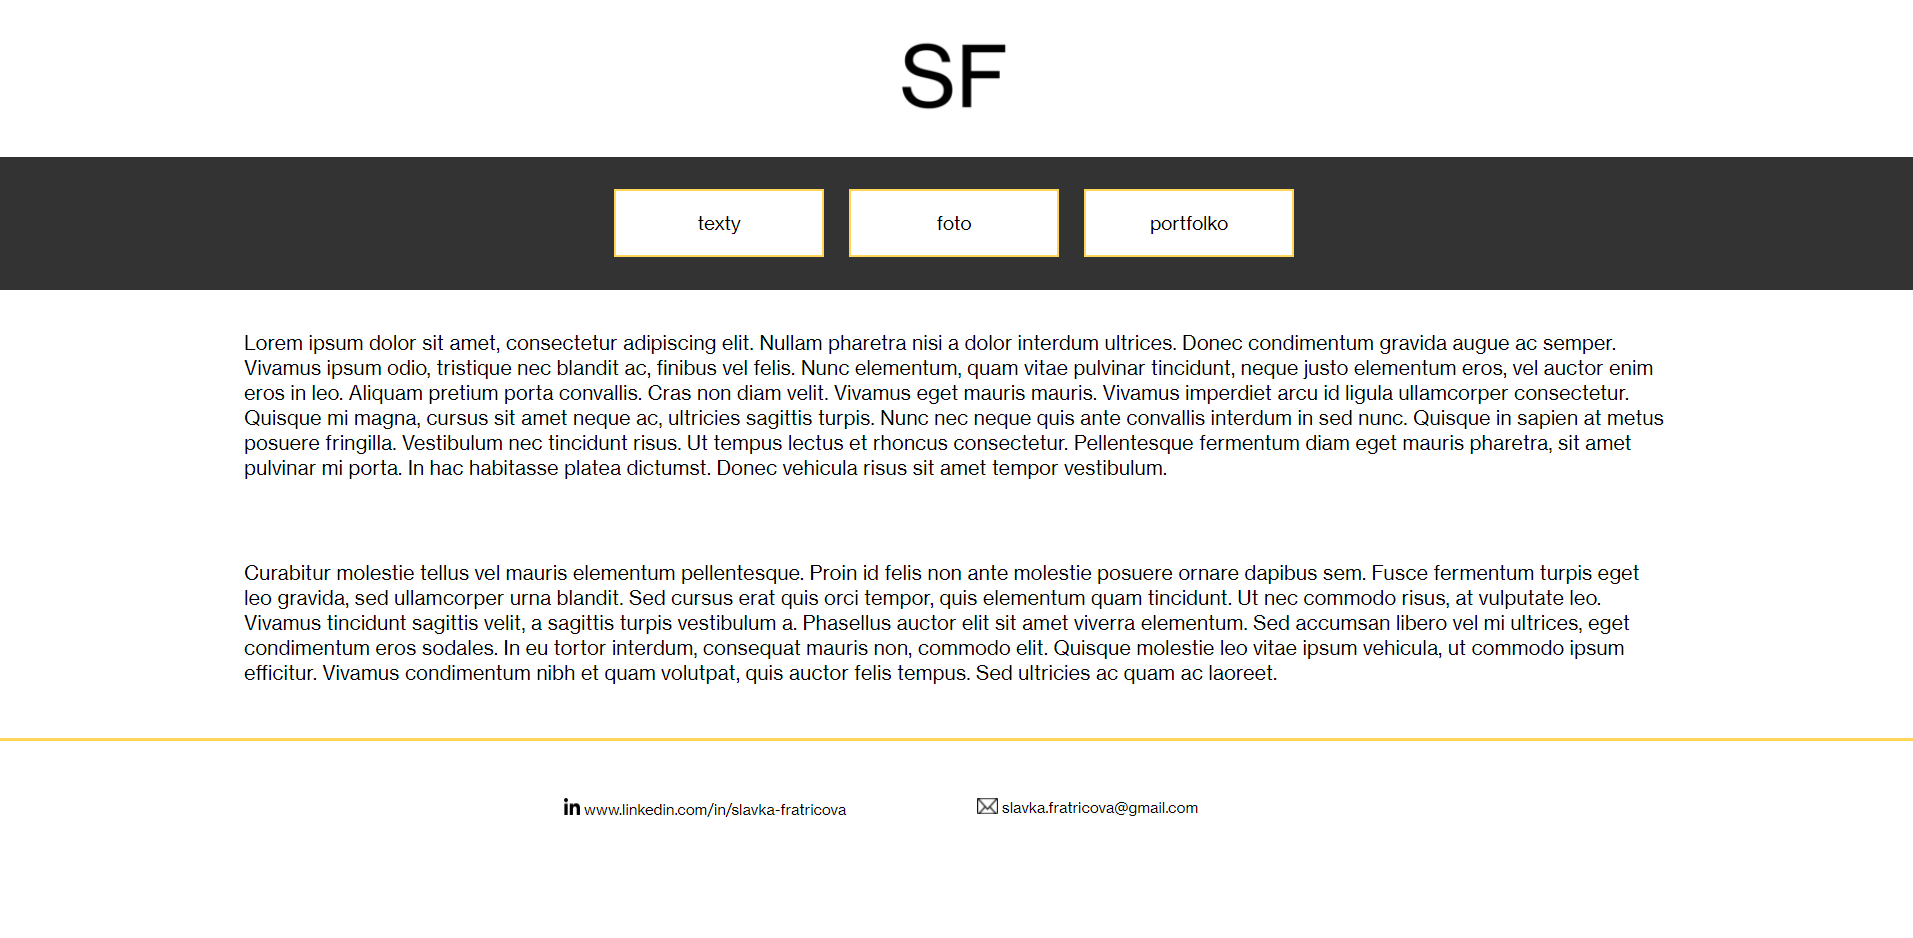
\includegraphics[width=\textwidth]{obr/uvodka.png}}
\caption{Úvodná stránka index.php.}\label{OBRAZOK 1.1}
\end{figure}

\vspace{4cm}

V časti texty, na podstránke indexx.php, nájde užívateľ nadpis a dátum publikácie článkov obr.\ref{OBRAZOK 1.2}. Po kliknutí na nadpis, sa užívateľovi zobrazí len požadovaný článok, ktorý sa rozvynie a zobrazí v celej dĺžke obr.\ref{OBRAZOK 1.3}.

\begin{figure}[!tbh]
\centering
\setlength{\fboxsep}{0pt}%
\setlength{\fboxrule}{1pt}%
\fbox{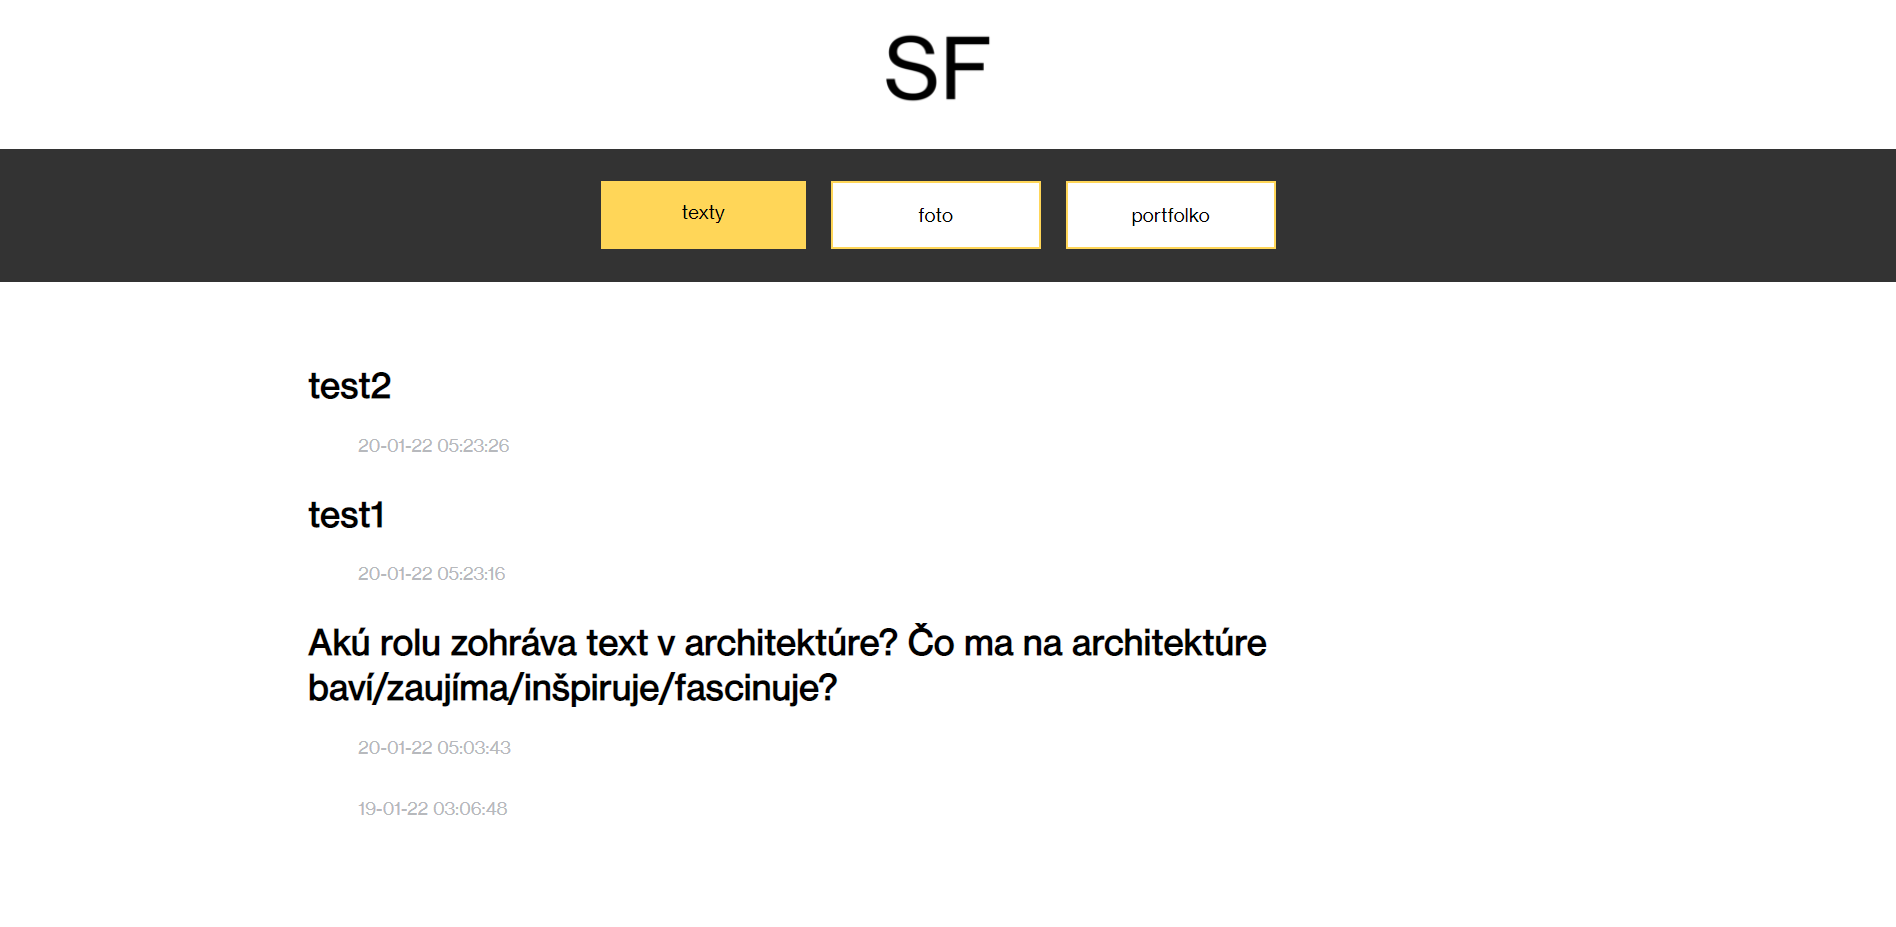
\includegraphics[width=\textwidth]{obr/texty_bez_text.png}}
\caption{Texty publikované na podstránke indexx.php.}\label{OBRAZOK 1.2}
\end{figure}

\begin{figure}[!tbh]
\centering
\setlength{\fboxsep}{0pt}%
\setlength{\fboxrule}{1pt}%
\fbox{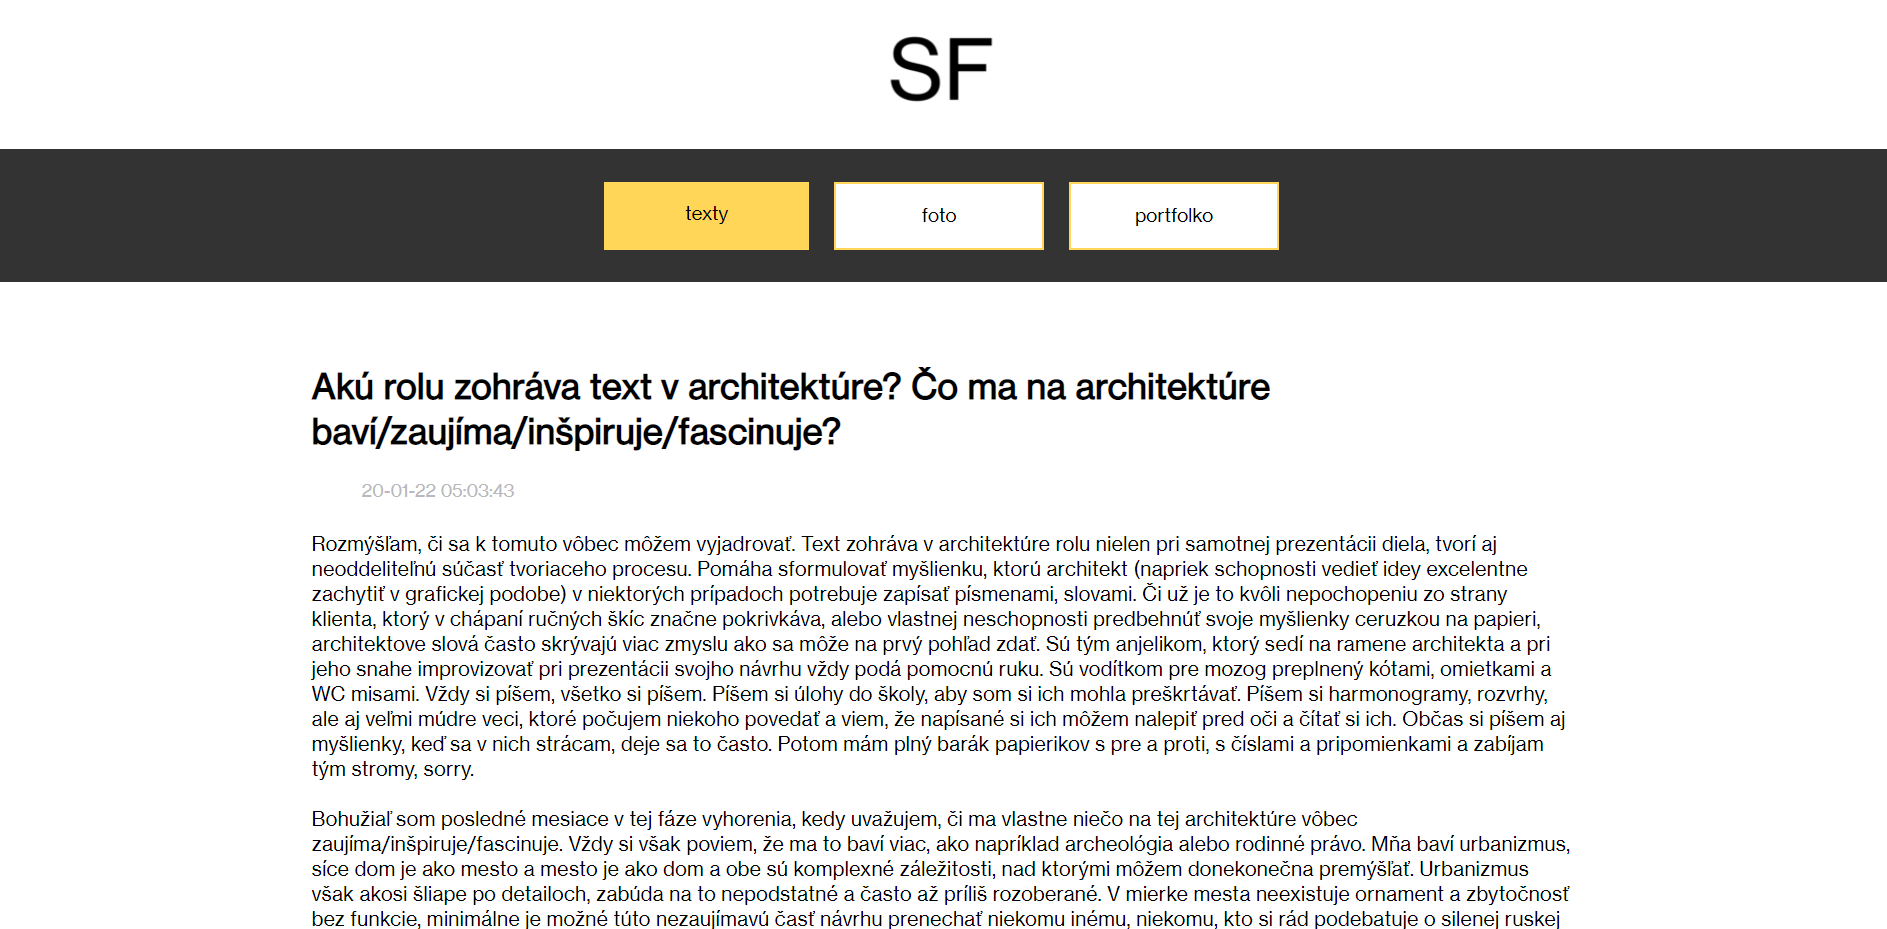
\includegraphics[width=\textwidth]{obr/texty_s_text.png}}
\caption{Zobrazenie konkrétneho textu na podstránke indexx.php.}\label{OBRAZOK 1.3}
\end{figure}


\section{Funkcie stránky}

\section{Fungovanie stránky}

\subsection{Súbory tvoriace stránku}

\subsection{Tvorba databázy pre stránku}

\subsection{Štruktúra stránky}